\clearpage
\section{Design of the FeedApp Prototype}
\label{sec:design}

The overall design framework for the FeedApp project was pre-established at the beginning of the assignment. This design was further amplified through the course of various lectures that looked into different aspects of the project.  Given our initial unfamiliarity with many of the technologies outlined in the project's scope, we proceeded to adopt those specified in the project guidelines.

The project's brief did offer the option to incorporate one additional technology, which, while seemingly providing a degree of flexibility, also imposed certain constraints on our technological explorations. For example, questions such as the feasibility of implementing the project in Python, the existence of a Python persistence model, or Python's capability to interface effectively with a database, remained unexplored. These potential avenues of inquiry could have provided a valabue alternative allowong a more complex design and quicker development approach.

However, the intensive and time-consuming nature of the assignments precluded a thorough investigation into these alternative technological possibilities. As a result, the project proceeded within the confines of the pre-specified technology stack, leaving some questions about potential alternative implementations and technologies unanswered.

\subsection{Architectural Overview} 

 Our foundational concept of the FeedApp application was to mimic some of the Kahoot application capabilities while remaining simplistic.  It is accessible through web browsers, ensuring compatibility with devices such as smartphones, tablets, and computers.  Key features of the FeedApp are listed below:

(rewrite so that each point is described in a full sentence)
\begin{enumerate}
\item Ability to create and particpate in polls
\item Flexibility to cast votes via an IoT device or a web browser. 
\item Real-time display of voting results and analytics.
\item Third Party access to data for analytics
\item User Authentication
\end{enumerate}

\subsection{Domain Model} 

Our domain model of the FeedApp, is represented in a Unified Modeling Language (UML) class diagram representing the fundamental objects and their relationships. By doing this we describe  behavior and functions in a clear way so that we are all on the same page.  Throughout the development lifecycle of the FeedApp, this domain model has undergone iterative modifications. These adaptations were essential to maintain alignment with changes made in our objectives.  A primary focus during these modifications has been the preservation of simplicity within the system's architecture. By continuously refining the domain model, we have ensured that the FeedApp remains functionally efficient.

\subsubsection{Users}
The domain model describes an entity of a user and categorizes it into two distinct types based on account registration status.  Users with registered accounts are granted full access within the FeedApp including the capability to create and participate in both public and private polls.  This category of user must undergo an authentication process which is described in TODO:Section.  Users without registerd accounts are only allowed to participate in publicly accessible  polls.  This restriction is a delibarate choice, allwoing our development efforts to maintain simpliciy in implementation.  

\subsubsection{Polls}
A key feature of the system is the poll entity, characterized by distinct attributes such as a title, an identification number, and the option to be set as private or public. Each poll is required to have a time limit and are also designed to integrate with Internet of Things (IoT) devices.  Furthermore, polls are designed to be flexible, allowing an unrestricted number of questions. The application does not impose a limit on the quantity of questions per poll.  In addition to this, for private polls, there is a feature to specify a list of authorized users who are permitted to vote. 
In the design of polls, the questions must be structured as binary-choice and closed-ended.  This format restricts responses to one of two predetermined options, exemplified by pairs such as True/False, Yes/No, or Pancakes/Waffles.  While the application does not impose time limits on individual questions, it integrates time restrictions at the poll level.  This design choice, made for ensuring simplicity in implementation, focuses on the entire poll rather than individual questions.

\subsubsection{IOTDevice}
For this project, a physical IoT device was chosen to add the interactive dimension to the polling process.  This device is intentionally simplistic, capable only of transmitting voting data without knowledge of the specific poll or question involved.  It operates via a Mosquitto broker, which relays messages from the IoT device to the feed application. The integration with the IoT device is minimalistic. The device's primary function is to acknowledge a voting action and communicate this to the feed application. It is not equipped to discern details about the poll or the voting options. The absence of an on-device display is compensated for by using a command-line interface to indicate when a vote has been cast. This setup was demonstrated in the submitted video, showcasing the Mosquitto broker's role in facilitating communication between the IoT device and the feed application.

\subsubsection{IOTDisplay}
The project's infrastructure includes an Internet of Things (IoT) device, functioning independently on a dedicated hardware platform. This device establishes a wireless connection with a Windows-based HP laptop, which serves a dual purpose: as a control unit and as a display for the IoT device's operations. The design stipulates that both the IoT device and the laptop must share the same Wi-Fi network for seamless communication.

\subsubsection{IOTDevice Integration with FeedApp}
Further enhancing the system's architecture is the incorporation of a Linux virtual machine (VM) on the HP laptop. This VM is designated as the application server, managing the core functionalities of the feedback feed application. Notably, the VM's connectivity is not restricted to the same Wi-Fi network as the IoT device, offering flexibility in network configurations. It communicates with the IoT device through a Mosquitto broker, which acts as an intermediary in message transmission. The IP address of the Mosquitto broker is hardcoded into the system for consistent connectivity.

The application leverages a REST API to handle incoming data from the IoT device. When a user interacts with the IoT device, such as by pressing a button, this action triggers a message that is relayed by the Mosquitto broker to the feed application. The application's REST API is configured to recognize this input, determining the active poll and the specific question being addressed by the IoT device. While the mechanism for transitioning between different poll questions was not fully established, the conceptual framework suggests that the REST API would facilitate this progression by incrementally recording votes and navigating to subsequent questions.

\subsubsection{Analytics}
Once the a vote is cast on the last quesiton in the poll, the application is designed to immediately reflect the analytical data offering insight into collective responses.  The system is designed to facilitate the display of analytics for all polls, regardless of their current status (active or inactive).  This functionality is implemented through a standardized display template, which is accessible via web browsers. The template ensures uniformity in the visualization of analytics, providing a coherent and consistent user experience. In addtion, the system's architecture allows for third-party applications to access poll-related data.  This capability enables external entities to conduct their own analytical assessments.  However, it is important to note that the scope of data accessible to third-party applications is confined to poll-level information. Granular data pertaining to individual questions within the polls is not available for external analysis.

\clearpage
\subsection{FrontEnd Design} 
To get an overview of how we wanted to implement the user interface, an application flow diagram was modeled. 
The diagram displays how the user navigates through the different frames in the front end of the application:

\begin{figure}[h]
  \centering
  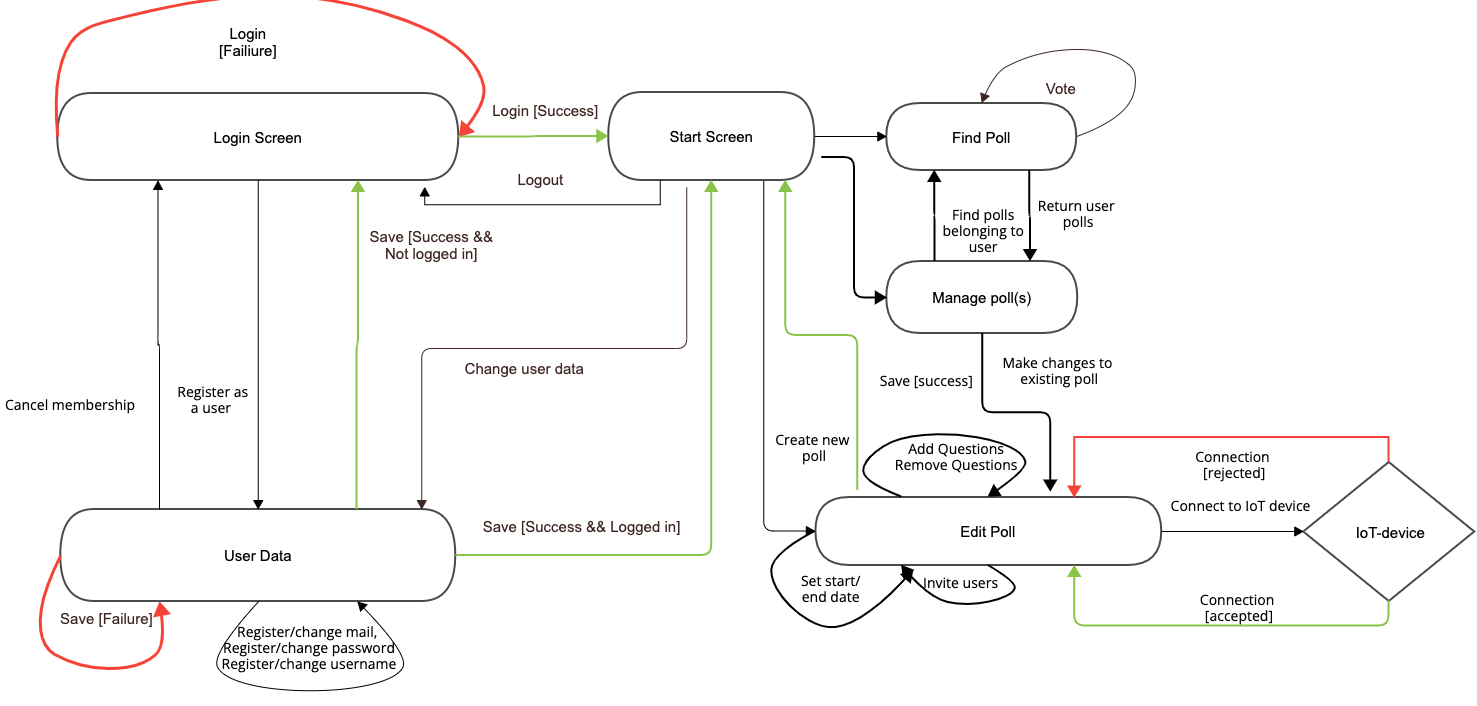
\includegraphics[scale=0.30]{figs/Application Flow Diagram (1).png}
  \caption{Application Flow Diagram}
  \label{fig:appFlow}
\end{figure}

Each screen has in the diagram been modelled as a state, and for every state, the user is able to do some action or provide some input. 
These actions or inputs are modelled as transitions, and are in the figure above illustrated with arrows. Transitions that results in errors are 
colored red, and transitions that does not result in errors are colored green. Our application consists of six screens. We have a login screen, 
where the user can either login, or create a new user. Once the user is logged in, he is directed to a start screen, where he gets the option to 
do multiple actions. He can search for a poll, which then can be voted on, or he can view and manage his own polls. He can create new polls,
and in this state he gets the option to pair the poll with an IoT device. 

The example below shows how you may include code. There are similar
styles for many other langages - in case you do not use Java in your
project. You can wrap the listing into a figure in case you need to
refer to it. How to create a figure was shown in Section~\ref{sec:technology}.

\lstinputlisting[language=java]{code/BoksVolum.java}
